\documentclass{beamer}

\usetheme{PSY9511}

\usepackage{listings}
\usepackage{pgfplots}

\usepgfplotslibrary{fillbetween}

\usetikzlibrary{arrows.meta}
\usetikzlibrary{calc}
\usetikzlibrary{patterns}

% Define settings for the listings package
\lstset{
    language=Python,
    basicstyle=\ttfamily\footnotesize,
    keywordstyle=\color{green},
    commentstyle=\color{purple},
    stringstyle=\color{orange},
    frame=shadowbox,
    breaklines=true
}


\title{Generativ KI i programmeringskurs}
\subtitle{KI for undervisning og vurdering på SV-fakultetet}
\author{Esten H. Leonardsen}
\date{\today}

\colorlet{cases}{red}
\colorlet{controls}{blue}

\begin{document}
	\begin{frame}
	 	\titlepage
	\end{frame}

	\begin{frame}{Fagbakgrunn}
		\begin{tabular}{l l}
			\textbullet\hspace{0.1cm}2011-2016&Mastergrad i Informatikk\\
			\textbullet\hspace{0.1cm}2016-2019&Softwareutvikler og analytiker i industrien\\
			\textbullet\hspace{0.1cm}2019-2024&Doktorgrad i Psykologi\\
			\textbullet\hspace{0.1cm}2024-&Post-doktor på psykologisk institutt\\
			&\small{- Foreleser "PSY9511: Maskinlæring"}\\
			&\small{- Veileder bachelor/master/PhD}\\
		\end{tabular}
	\end{frame}

	\begin{frame}{Bruksområder}
		\begin{tikzpicture}
			\node[] at (-5.25, -3.5) {};
			\node[] at (5.25, 3.5) {};

			\only<1>{
				\node[text width=10cm] at (0, 0) {
					\begin{enumerate}
						\item Utforming av grafikk/slides
						\item Støtte til oppgaveformuleringer
						\item Oppfordret studentene til å teste KI i sitt arbeid
					\end{enumerate}
				};
			}

			\only<2>{
				\node[inner sep=0pt, draw=black] at (0, 0) {
					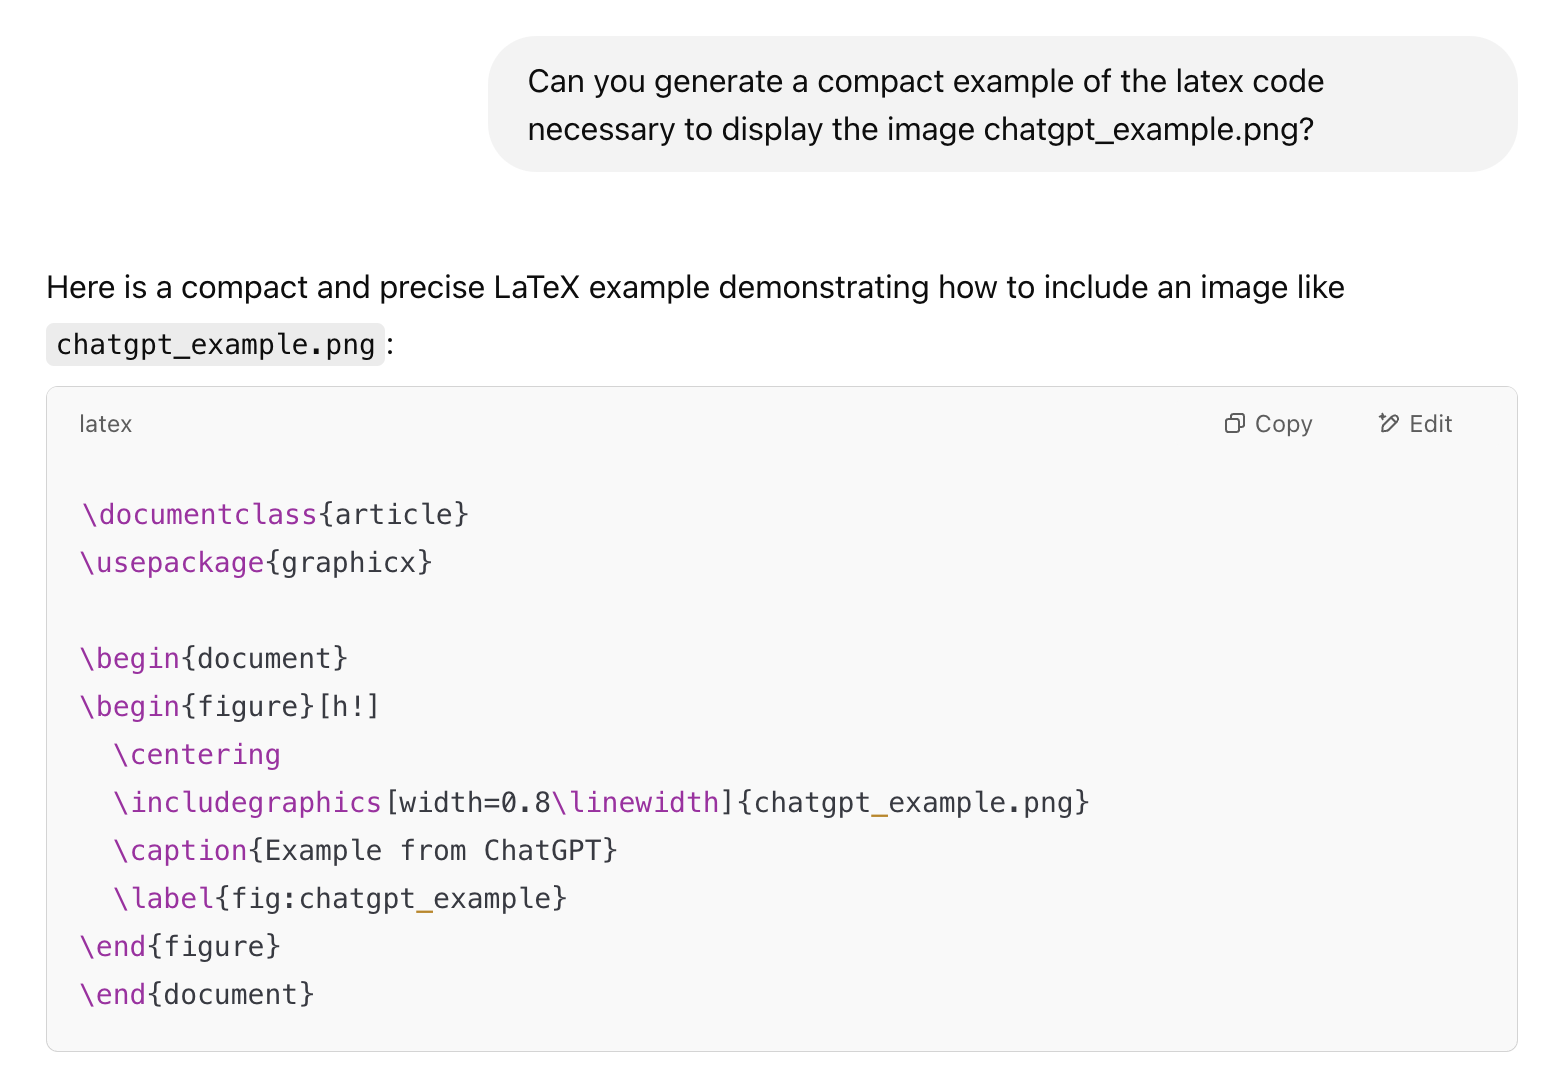
\includegraphics[width=9.5cm]{data/chatgpt_example.png}
				};
			}

			\only<3>{
				\node[font=\scriptsize] at (0, 0) {
					\url{https://chatgpt.com/c/67e95f86-538c-8013-a01d-4e057aa2a56d}
				};
			}

			\only<4>{
				\node[font=\scriptsize] at (0, 0) {
					\url{https://uio.instructure.com/courses/54846/assignments/127687}
				};
			}
			\only<5>{
				\node[font=\scriptsize] at (0, 0) {
					\url{https://uio.instructure.com/courses/54846/assignments/128391}
				};
			}
		\end{tikzpicture}
	\end{frame}
	\begin{frame}{Generativ KI i moderne programmering}
		\begin{tikzpicture}
			\node[] at (-5.25, -3.5) {};
			\node[] at (5.25, 3.5) {};

			\only<1>{
				\node[inner sep=0pt, draw=black] (cursor) at (0, 1) {
					
\includegraphics[width=11cm]{data/cursor.png}
				};
				\node[anchor=north, inner sep=8pt] at (cursor.south) {
					\url{https://www.cursor.com/}
				};
			}
			\visible<2-3>{
				\node[font=\tiny, anchor=south, text width=10.5cm, align=flush center] at (0, -3.85) {Kalliamvakou, E. (2022). \textit{Research: quantifying GitHub Copilot’s impact on developer productivity and happiness}. The GitHub Blog};
			}
			\only<2>{
				\node[inner sep=0pt, draw=black] at (0, 0) {
					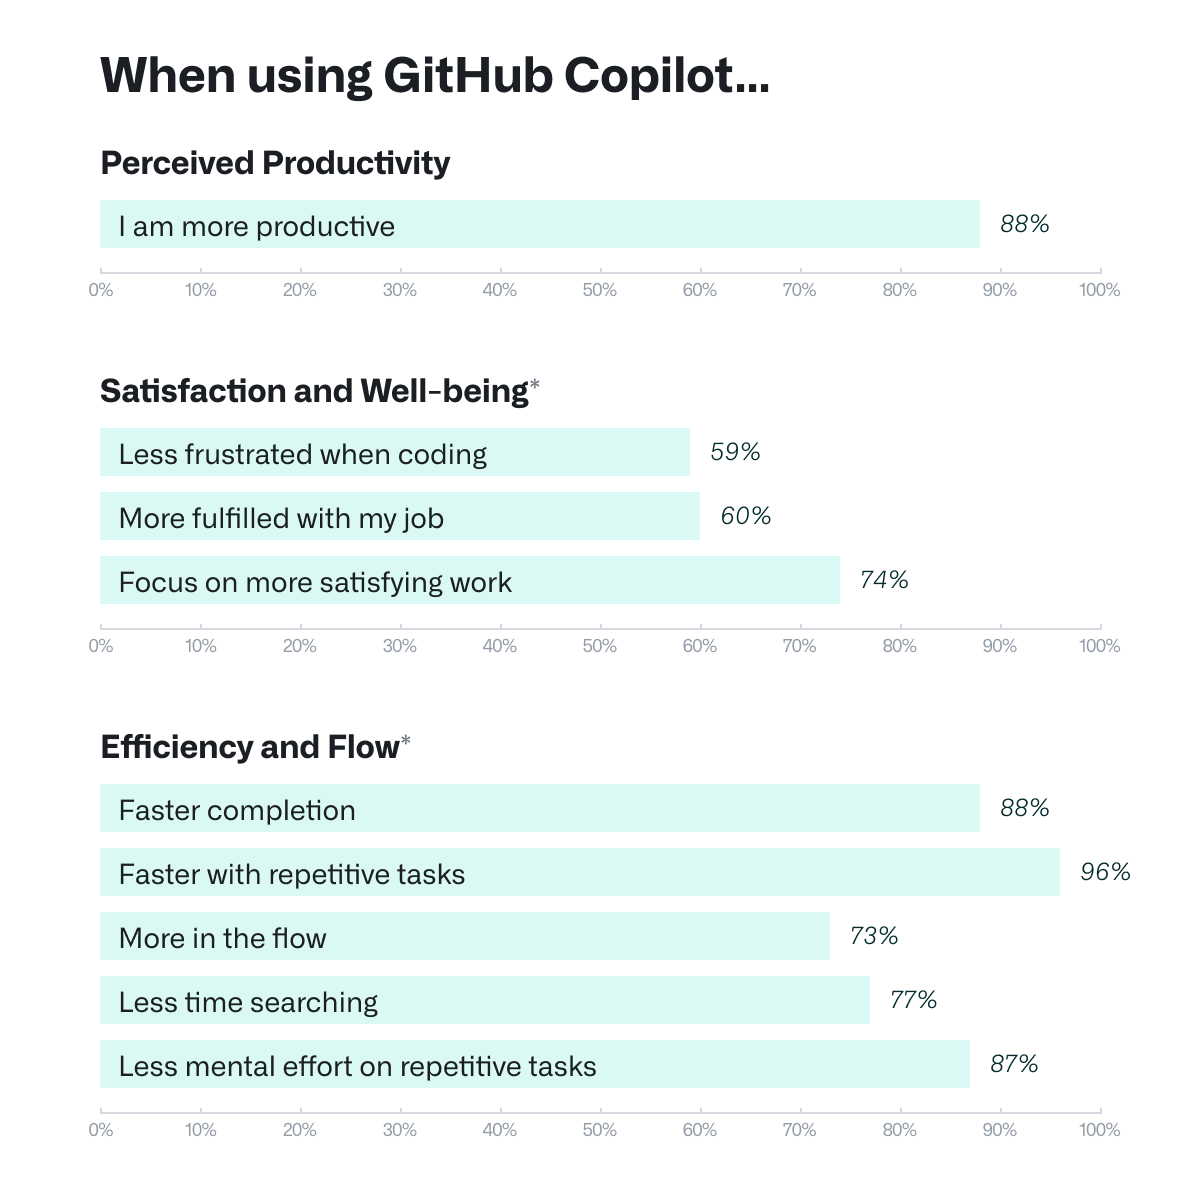
\includegraphics[width=5.5cm]{data/copilot1.png}
				};
			}
			\only<3>{
				\node[inner sep=0pt, draw=black] at (0, 0) {
					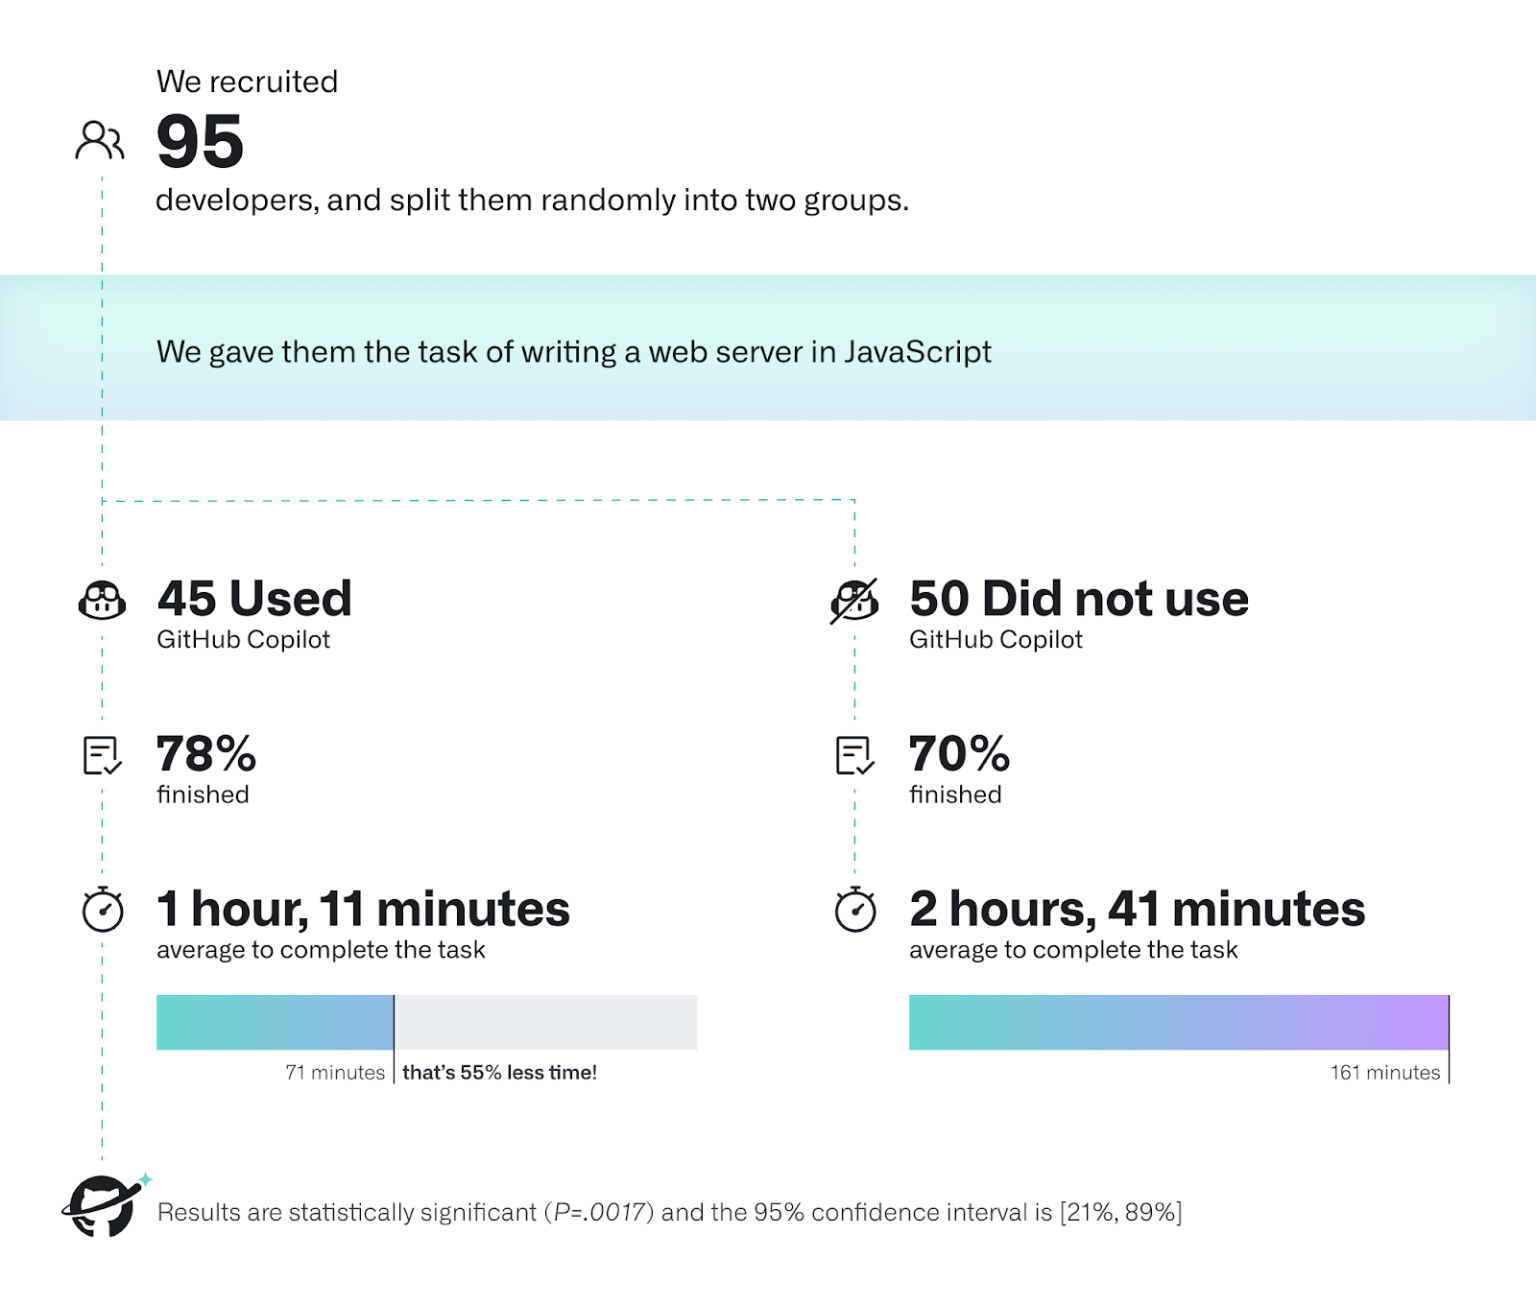
\includegraphics[width=6.5cm]{data/copilot2.png}
				};
			}
		\end{tikzpicture}
	\end{frame}

	\begin{frame}[fragile]{Generativ AI i PSY9511}
		\begin{tikzpicture}
			\node[] at (-5.25, -3.5) {};
			\node[] at (5.25, 3.5) {};

			\only<1>{
				\node[inner sep=0pt, draw=black] at (0, 0) {
					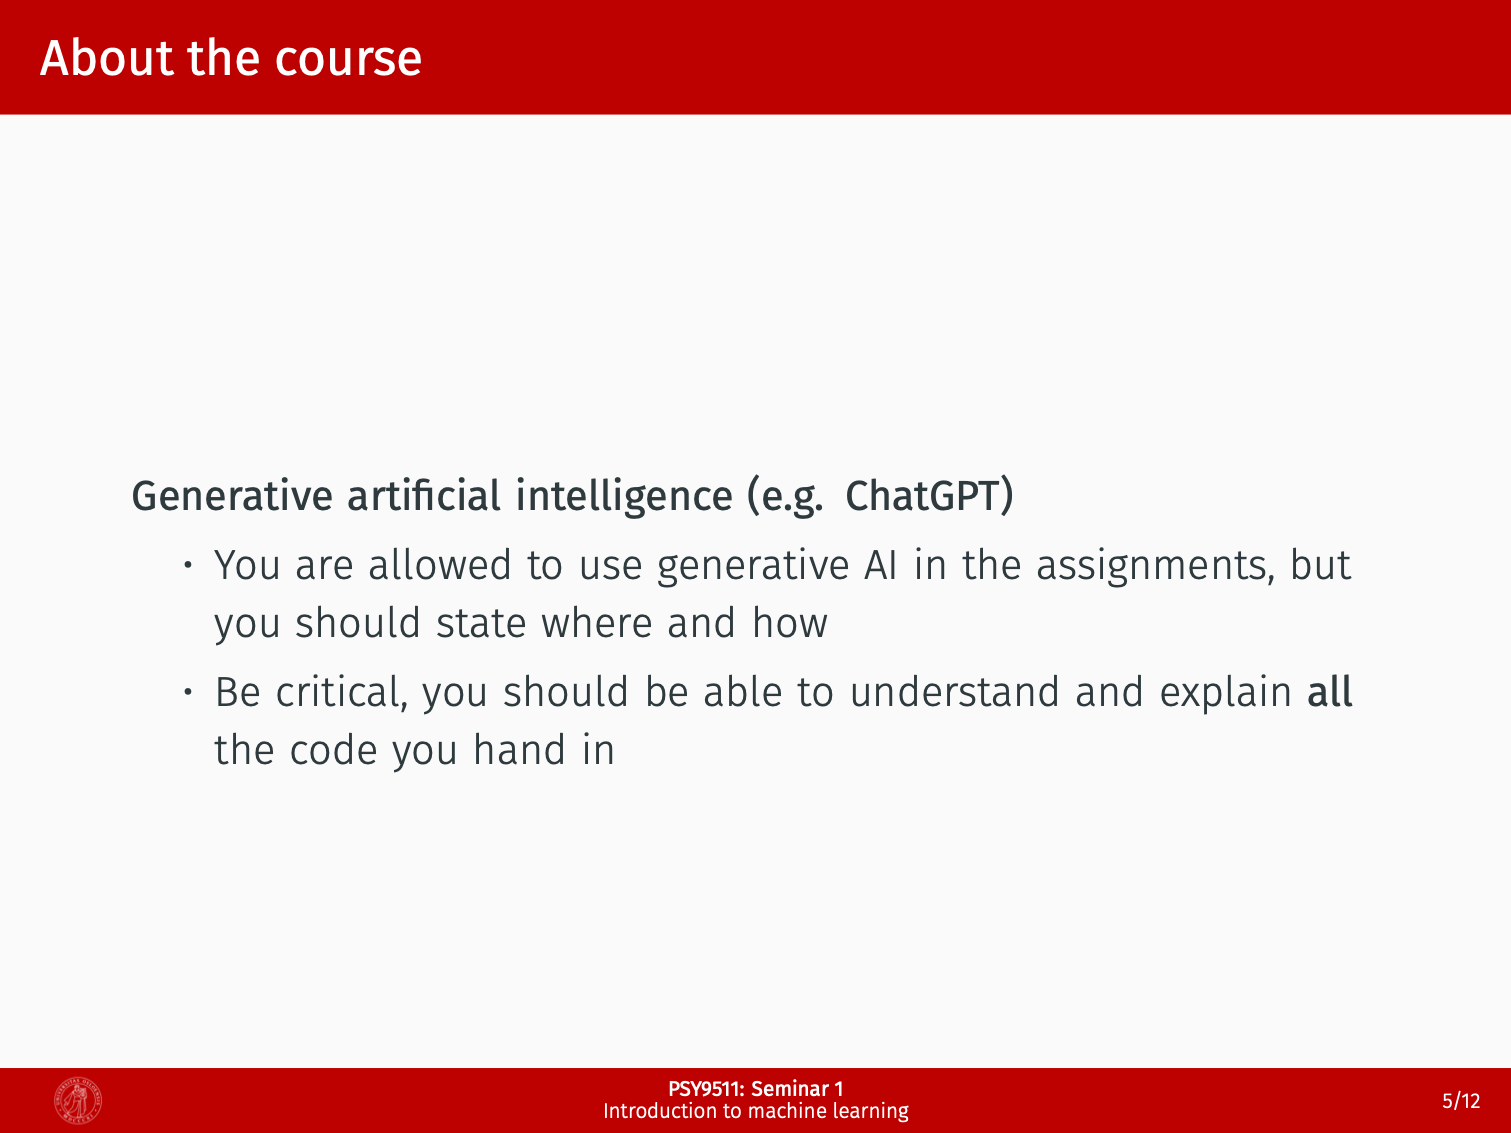
\includegraphics[width=8cm]{data/intro.png}
				};
			}

			\only<2>{
				\PythonInputNode{1}{(-5, 3)}{pythonnode}{9.5cm}{7}{
					\# Attempt 1^^J
					\#def sum_of_squares(n):^^J
					\#{ }{ }{ }{ }total = 0^^J
					\#{ }{ }{ }{ }for i in range(1, n):^^J
					\#{ }{ }{ }{ }{ }{ }{ }{ }total += i * i^^J
					\#{ }{ }{ }{ }return total^^J
					^^J
					\# Attempt 2^^J
					\#def sum_of_squares(n):^^J
					\#{ }{ }{ }{ }total = 0^^J
					\#{ }{ }{ }{ }for i in range(n):^^J
					\#{ }{ }{ }{ }{ }{ }{ }{ }total += i * i^^J
					\#{ }{ }{ }{ }return total^^J
					^^J
					\# Attempt 3^^J
					def sum_of_squares(n):^^J
					{ }{ }{ }{ }total = 0^^J
					{ }{ }{ }{ }for i in range(1, n+1):^^J
					{ }{ }{ }{ }{ }{ }{ }{ }total = i * i^^J
					{ }{ }{ }{ }return total^^J
                }
			}

			\only<3-4>{
				\node[inner sep=0pt, draw=black] at (0, 1.5) {
					
\includegraphics[scale=0.4]{data/reddit1.png}
				};
			}
			\only<4>{
				\node[inner sep=0pt, draw=black] at (0, -2) {
					
\includegraphics[scale=0.4]{data/reddit2.png}
				};
			}
		\end{tikzpicture}
	\end{frame}

	\begin{frame}{Erfaring med generativ KI}
		\begin{itemize}
		\item Oppfordrer til å bruke generativ KI i oppgaver (kun siste semester)
		\item Har sett en økning i kvaliteten på innleveringene (men usikker på hvor relatert dette er)
		\item Studenter er tilbakeholdne med å snakke om at de bruker generativ KI (dersom de gjør det)
		\item Noen innleveringer vitner om feilaktig og lite reflektert bruk av generativ KI (selv om det har vært mindre etter den eksplisitte oppfordringen med rammer)
		\end{itemize}
	\end{frame}
\end{document}
